% Options for packages loaded elsewhere
\PassOptionsToPackage{unicode}{hyperref}
\PassOptionsToPackage{hyphens}{url}
\PassOptionsToPackage{dvipsnames,svgnames,x11names}{xcolor}
%
\documentclass[
  letterpaper,
  DIV=11,
  numbers=noendperiod]{scrartcl}

\usepackage{amsmath,amssymb}
\usepackage{lmodern}
\usepackage{iftex}
\ifPDFTeX
  \usepackage[T1]{fontenc}
  \usepackage[utf8]{inputenc}
  \usepackage{textcomp} % provide euro and other symbols
\else % if luatex or xetex
  \usepackage{unicode-math}
  \defaultfontfeatures{Scale=MatchLowercase}
  \defaultfontfeatures[\rmfamily]{Ligatures=TeX,Scale=1}
\fi
% Use upquote if available, for straight quotes in verbatim environments
\IfFileExists{upquote.sty}{\usepackage{upquote}}{}
\IfFileExists{microtype.sty}{% use microtype if available
  \usepackage[]{microtype}
  \UseMicrotypeSet[protrusion]{basicmath} % disable protrusion for tt fonts
}{}
\makeatletter
\@ifundefined{KOMAClassName}{% if non-KOMA class
  \IfFileExists{parskip.sty}{%
    \usepackage{parskip}
  }{% else
    \setlength{\parindent}{0pt}
    \setlength{\parskip}{6pt plus 2pt minus 1pt}}
}{% if KOMA class
  \KOMAoptions{parskip=half}}
\makeatother
\usepackage{xcolor}
\setlength{\emergencystretch}{3em} % prevent overfull lines
\setcounter{secnumdepth}{-\maxdimen} % remove section numbering
% Make \paragraph and \subparagraph free-standing
\ifx\paragraph\undefined\else
  \let\oldparagraph\paragraph
  \renewcommand{\paragraph}[1]{\oldparagraph{#1}\mbox{}}
\fi
\ifx\subparagraph\undefined\else
  \let\oldsubparagraph\subparagraph
  \renewcommand{\subparagraph}[1]{\oldsubparagraph{#1}\mbox{}}
\fi


\providecommand{\tightlist}{%
  \setlength{\itemsep}{0pt}\setlength{\parskip}{0pt}}\usepackage{longtable,booktabs,array}
\usepackage{calc} % for calculating minipage widths
% Correct order of tables after \paragraph or \subparagraph
\usepackage{etoolbox}
\makeatletter
\patchcmd\longtable{\par}{\if@noskipsec\mbox{}\fi\par}{}{}
\makeatother
% Allow footnotes in longtable head/foot
\IfFileExists{footnotehyper.sty}{\usepackage{footnotehyper}}{\usepackage{footnote}}
\makesavenoteenv{longtable}
\usepackage{graphicx}
\makeatletter
\def\maxwidth{\ifdim\Gin@nat@width>\linewidth\linewidth\else\Gin@nat@width\fi}
\def\maxheight{\ifdim\Gin@nat@height>\textheight\textheight\else\Gin@nat@height\fi}
\makeatother
% Scale images if necessary, so that they will not overflow the page
% margins by default, and it is still possible to overwrite the defaults
% using explicit options in \includegraphics[width, height, ...]{}
\setkeys{Gin}{width=\maxwidth,height=\maxheight,keepaspectratio}
% Set default figure placement to htbp
\makeatletter
\def\fps@figure{htbp}
\makeatother

\KOMAoption{captions}{tableheading}
\makeatletter
\makeatother
\makeatletter
\makeatother
\makeatletter
\@ifpackageloaded{caption}{}{\usepackage{caption}}
\AtBeginDocument{%
\ifdefined\contentsname
  \renewcommand*\contentsname{Table of contents}
\else
  \newcommand\contentsname{Table of contents}
\fi
\ifdefined\listfigurename
  \renewcommand*\listfigurename{List of Figures}
\else
  \newcommand\listfigurename{List of Figures}
\fi
\ifdefined\listtablename
  \renewcommand*\listtablename{List of Tables}
\else
  \newcommand\listtablename{List of Tables}
\fi
\ifdefined\figurename
  \renewcommand*\figurename{Figure}
\else
  \newcommand\figurename{Figure}
\fi
\ifdefined\tablename
  \renewcommand*\tablename{Table}
\else
  \newcommand\tablename{Table}
\fi
}
\@ifpackageloaded{float}{}{\usepackage{float}}
\floatstyle{ruled}
\@ifundefined{c@chapter}{\newfloat{codelisting}{h}{lop}}{\newfloat{codelisting}{h}{lop}[chapter]}
\floatname{codelisting}{Listing}
\newcommand*\listoflistings{\listof{codelisting}{List of Listings}}
\makeatother
\makeatletter
\@ifpackageloaded{caption}{}{\usepackage{caption}}
\@ifpackageloaded{subcaption}{}{\usepackage{subcaption}}
\makeatother
\makeatletter
\@ifpackageloaded{tcolorbox}{}{\usepackage[many]{tcolorbox}}
\makeatother
\makeatletter
\@ifundefined{shadecolor}{\definecolor{shadecolor}{rgb}{.97, .97, .97}}
\makeatother
\makeatletter
\makeatother
\ifLuaTeX
  \usepackage{selnolig}  % disable illegal ligatures
\fi
\IfFileExists{bookmark.sty}{\usepackage{bookmark}}{\usepackage{hyperref}}
\IfFileExists{xurl.sty}{\usepackage{xurl}}{} % add URL line breaks if available
\urlstyle{same} % disable monospaced font for URLs
\hypersetup{
  colorlinks=true,
  linkcolor={blue},
  filecolor={Maroon},
  citecolor={Blue},
  urlcolor={Blue},
  pdfcreator={LaTeX via pandoc}}

\author{}
\date{}

\begin{document}
\ifdefined\Shaded\renewenvironment{Shaded}{\begin{tcolorbox}[interior hidden, borderline west={3pt}{0pt}{shadecolor}, frame hidden, sharp corners, enhanced, breakable, boxrule=0pt]}{\end{tcolorbox}}\fi

\hypertarget{intro}{%
\section{Intro}\label{intro}}

\begin{itemize}
\tightlist
\item
  Time series analysis often comes down to the question of causality:
  How did the past influence the future?
\item
  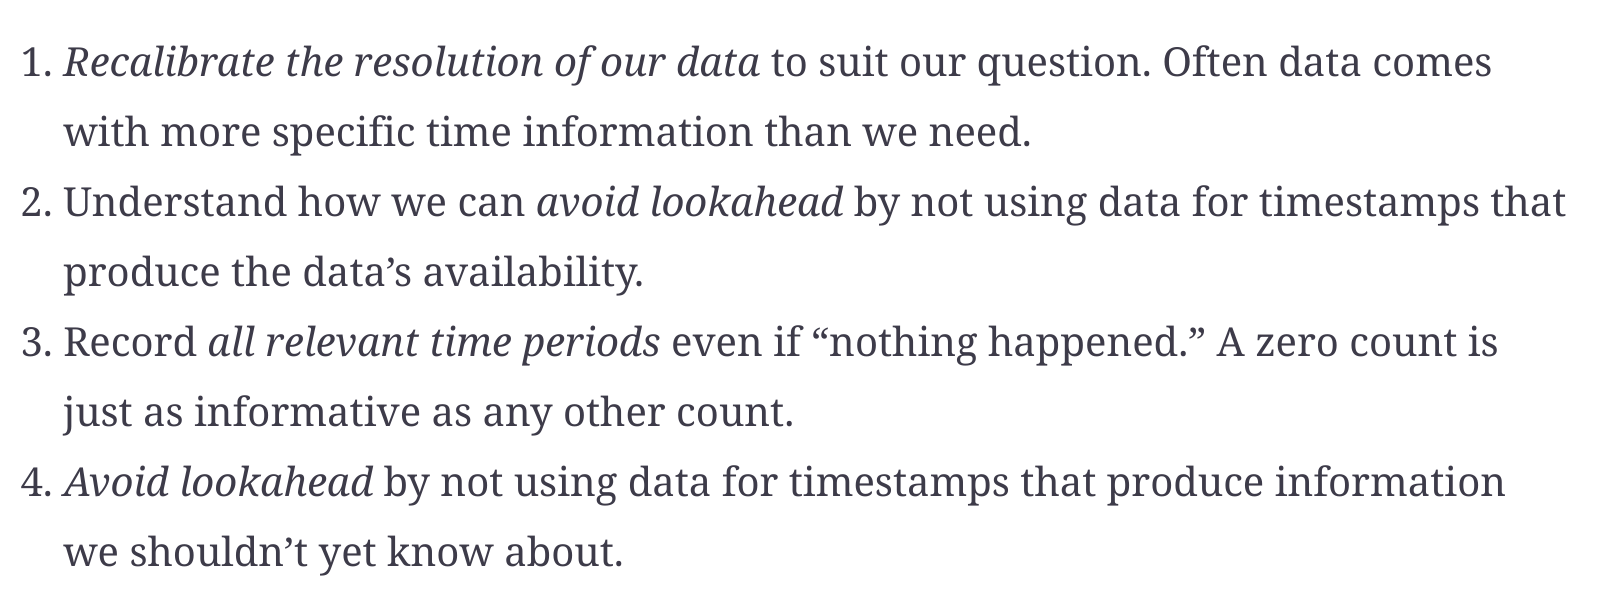
\includegraphics{/Images/time_series.png}
\end{itemize}

\hypertarget{timestamp-troubles}{%
\subsubsection{Timestamp troubles}\label{timestamp-troubles}}

\begin{itemize}
\tightlist
\item
  what process generated the timestamp, how and when
\item
  Time zone information
\item
  Record your own actions and see how they are captured
\item
  Local or universal time
\end{itemize}

\hypertarget{filling-missing-values}{%
\subsubsection{Filling missing values}\label{filling-missing-values}}

\begin{itemize}
\tightlist
\item
  Forward fill
\item
  Moving average of past values - use only the data that occurred before
  the missing data point
\item
  Interpolation - Determining the values of missing points based on
  geometric constraints regarding how we want the overall data to behave
\end{itemize}

\hypertarget{upsampling-and-downsampling}{%
\subsubsection{Upsampling and
downsampling}\label{upsampling-and-downsampling}}

\begin{itemize}
\tightlist
\item
  To match the frequency of different time series data
\item
  We either increase or decrease the timestamp frequency
\end{itemize}

\hypertarget{downsampling-the-data}{%
\paragraph{Downsampling the data}\label{downsampling-the-data}}

\begin{itemize}
\tightlist
\item
  The original resolution of the data isn't sensible
\item
  Match against data at a lower frequency - we can either downsample,
  take average, weighted mean etc.
\item
  Selecting out every nth element
\end{itemize}

\hypertarget{upsampling-the-data}{%
\paragraph{Upsampling the data}\label{upsampling-the-data}}

\begin{itemize}
\tightlist
\item
  convert irregularly sampled time series to a regularly timed one
\item
  Inputs sampled at different frequencies
\item
  Knowledge of time series dynamics - Treat as a missing data problem
  and missing data techniques can be applied.
\end{itemize}

\hypertarget{smoothing-data}{%
\paragraph{Smoothing data}\label{smoothing-data}}

\begin{itemize}
\item
  Moving average is used to eliminate measurement spikes, errors of
  measurement etc.
\item
  \textbf{purpose of smoothing}
\item
  Data preparation - Raw data unsuitable
\item
  Feature generation
\item
  Prediction - For many processes prediction is mean, which we get from
  a smoothed feature
\item
  Visualization - Add signal to a noisy plot
\item
  Exponential smoothing - All data points are not treated equally
\item
  More weight to recent data
\item
  \begin{figure}

  {\centering 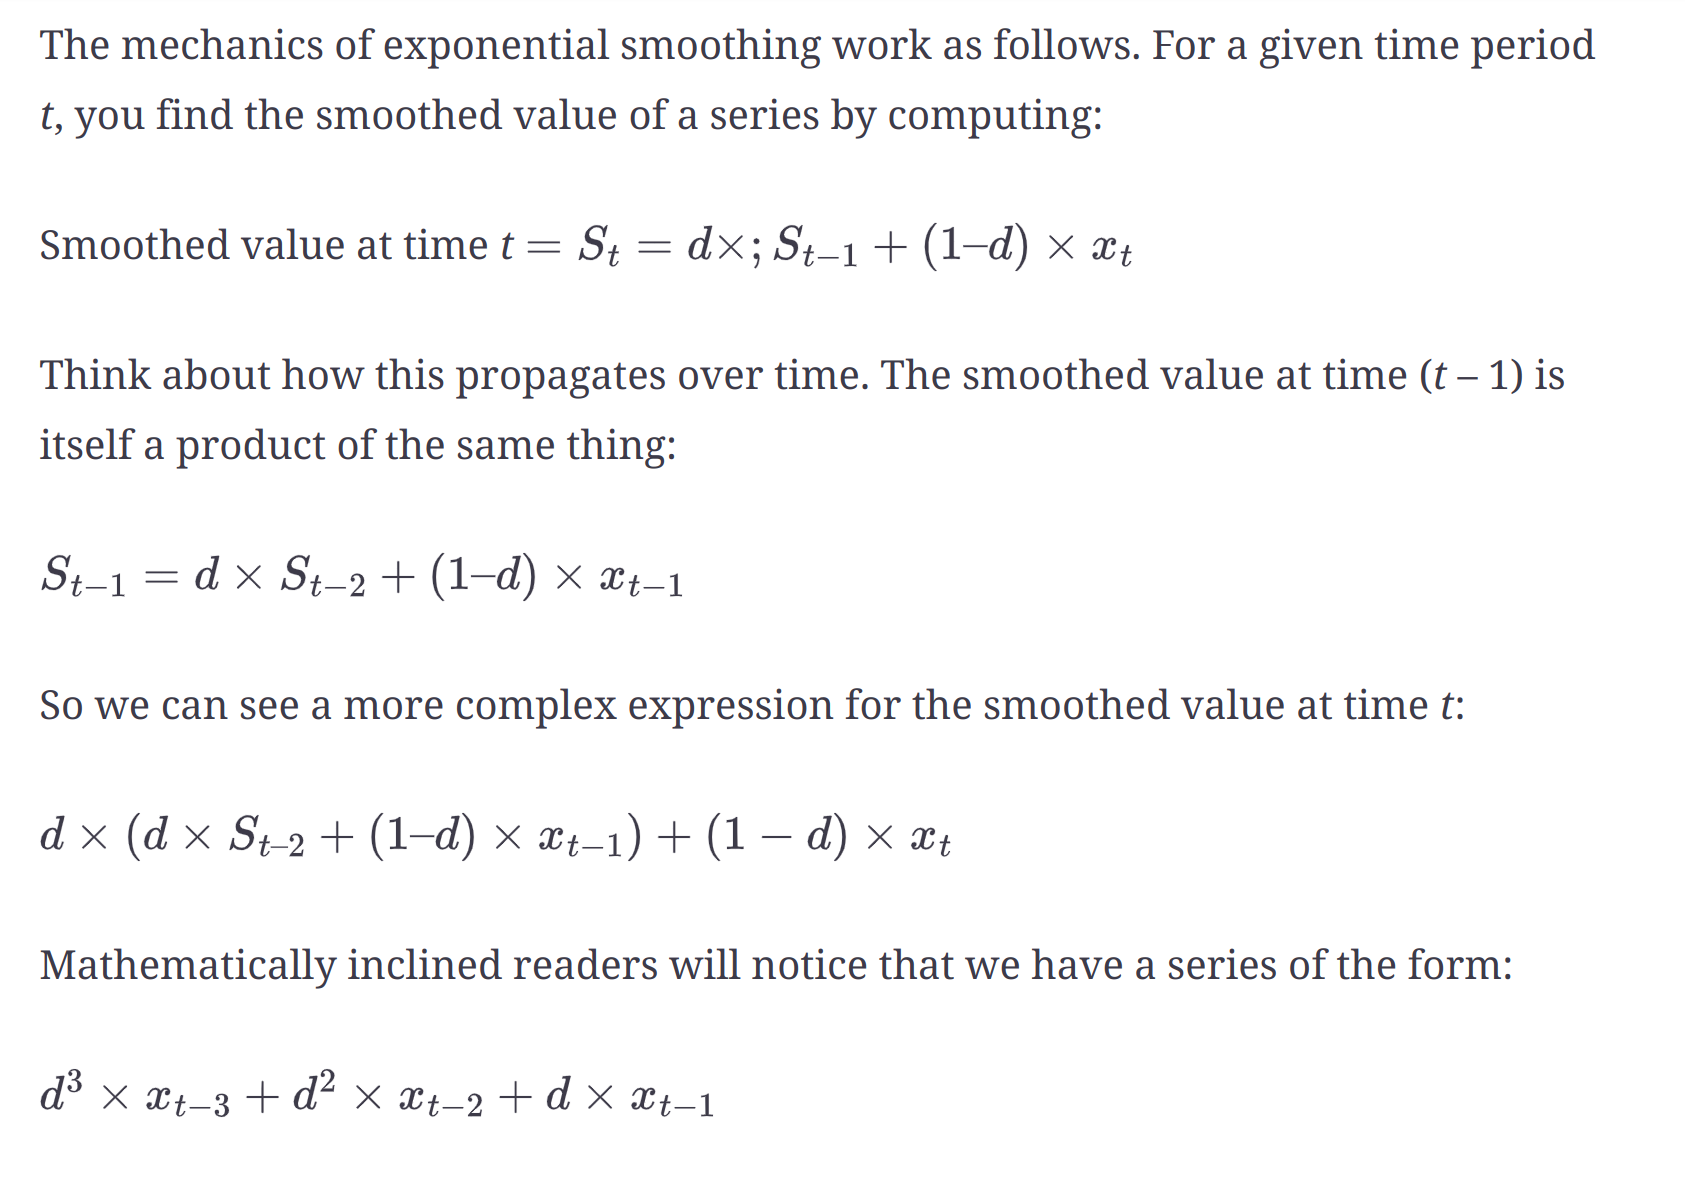
\includegraphics{/Images/exponential_smoothing.png}

  }

  \caption{Equation for exponential smoothing}

  \end{figure}
\item
  \begin{figure}

  {\centering 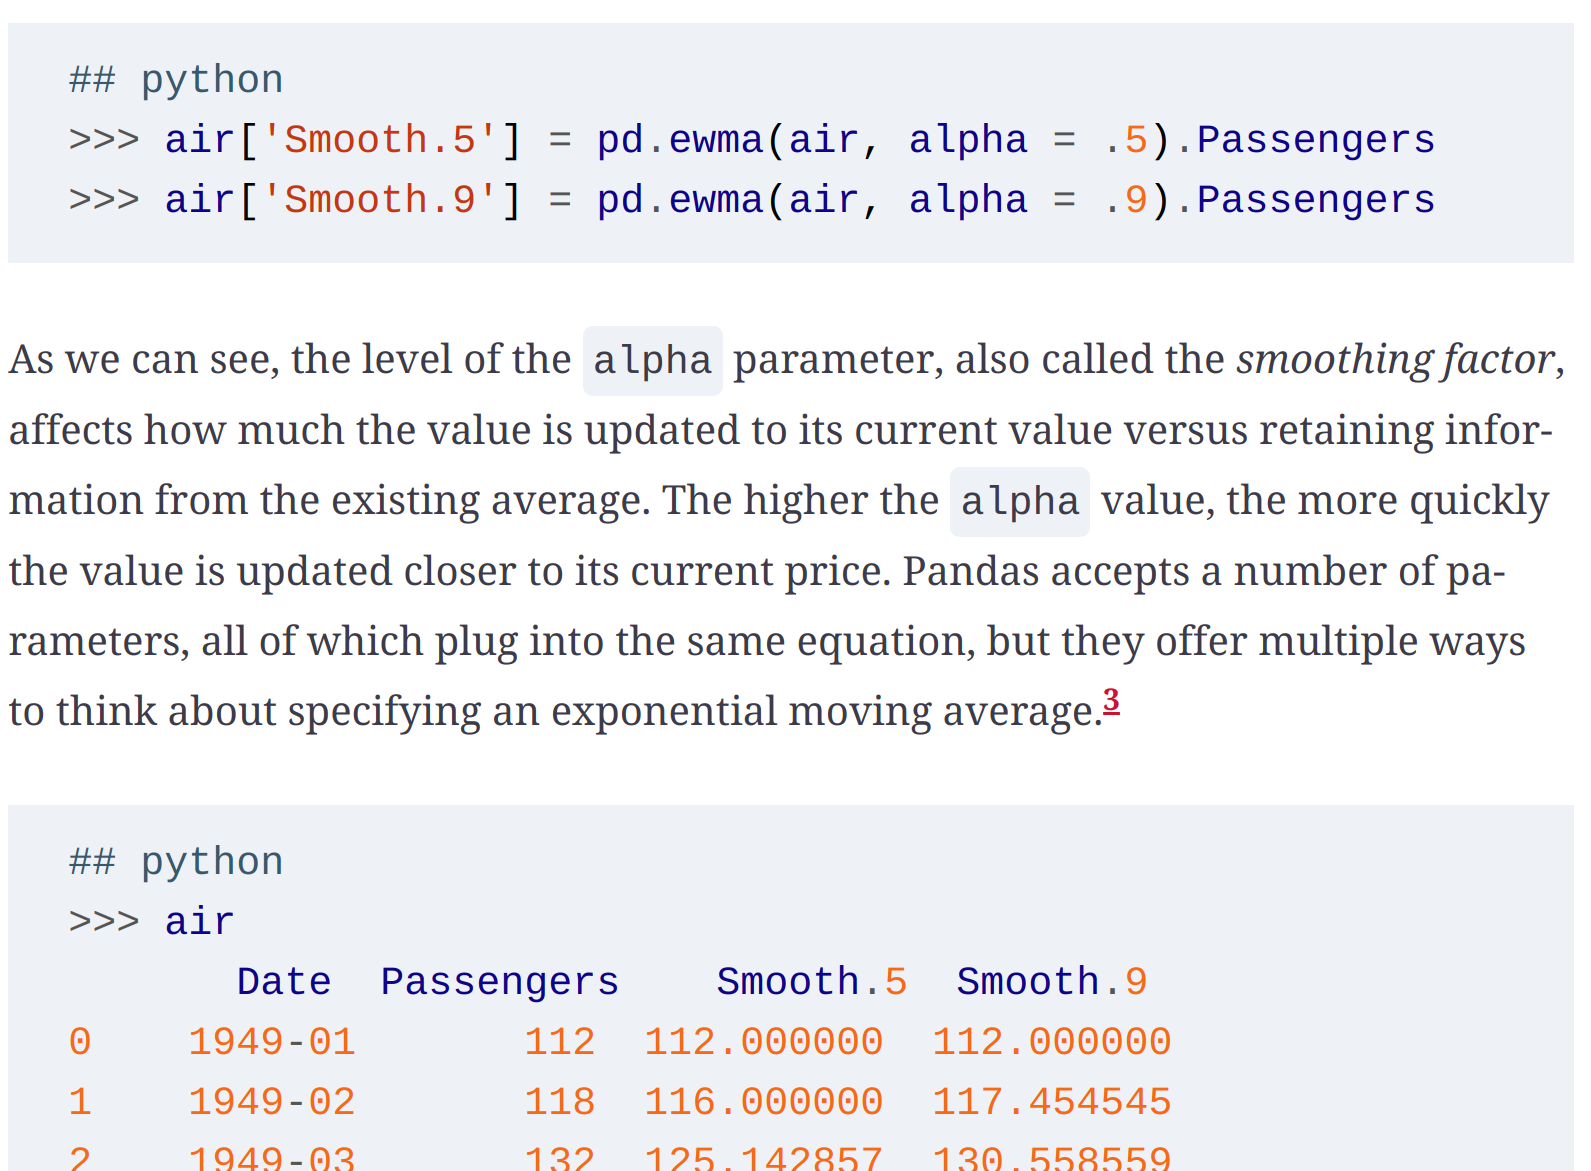
\includegraphics{/Images/smoothing_pandas.png}

  }

  \caption{Doing smoothing with pandas}

  \end{figure}
\item
  Exponential smoothing does not perform well in case of data with a
  long-term trend
\item
  Holt's method and holt-winters smoothing are two exponential smoothing
  methods applied to data with a trend or with a trend and a seasonality
\item
  Kalman filters and LOESS(locally estimated scatter plot smoothing) are
  other computationally involved methods - These methods leak
  information from the future - Not appropriate for forecasting
\item
  Smoothing is a commonly used form of forecasting, and you can use a
  smoothed time series (without lookahead) as one easy null model when
  you are testing whether a fancier method is actually producing a
  successful forecast
\end{itemize}

\hypertarget{seasonality}{%
\subsection{Seasonality}\label{seasonality}}

\begin{itemize}
\tightlist
\item
  Seasonal time series are time series in which behaviors recur over a
  fixed period. There can be multiple periodicities reflecting different
  tempos of seasonality, such as the seasonality of the 24-hour day
  versus the 12-month calendar season, both of which exhibit strong
  features in most time series relating to human behavior.
\end{itemize}

\hypertarget{time-zones}{%
\subsection{Time Zones}\label{time-zones}}

\begin{itemize}
\tightlist
\item
  Python libraries to deal with Timezone - datetime, pytz and dateutil
\end{itemize}

\begin{figure}

{\centering 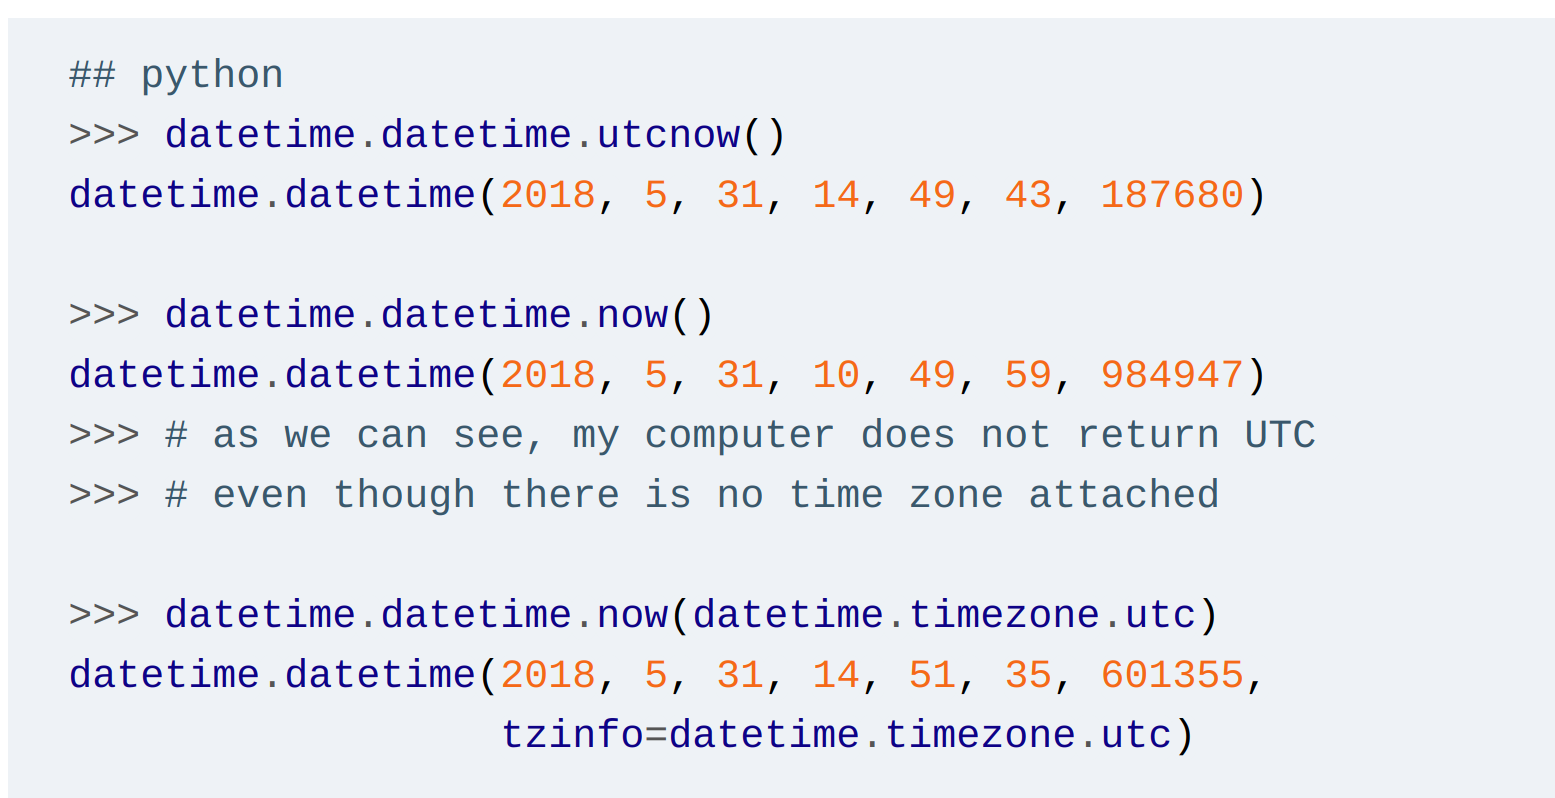
\includegraphics{/Images/timezone_python.png}

}

\caption{current time in python}

\end{figure}

\begin{itemize}
\tightlist
\item
  Be careful with timezone conversions
\item
  Dealing with daylight savings can be tricky
\end{itemize}

\hypertarget{lookahead}{%
\subsubsection{Lookahead}\label{lookahead}}

\begin{itemize}
\tightlist
\item
  Processing and cleaning time-related data can be a tedious and
  detail-oriented process.There is tremendous danger in data cleaning
  and processing of introducing a lookahead! You should have lookaheads
  only if they are intentional, and this is rarely appropriate.
\end{itemize}



\end{document}
